\documentclass[review]{elsarticle}

\usepackage{amsmath}
\usepackage{booktabs}
\usepackage{dirtytalk}
\usepackage{subcaption}
\usepackage{tabularx}
\usepackage{nicefrac}
\usepackage[usenames]{xcolor}
\usepackage{lineno,hyperref}
\modulolinenumbers[5]

\journal{Composites Part A}

%%%%%%%%%%%%%%%%%%%%%%%
%% Elsevier bibliography styles
%%%%%%%%%%%%%%%%%%%%%%%
%% To change the style, put a % in front of the second line of the current style and
%% remove the % from the second line of the style you would like to use.
%%%%%%%%%%%%%%%%%%%%%%%

%% Numbered
%\bibliographystyle{model1-num-names}

%% Numbered without titles
%\bibliographystyle{model1a-num-names}

%% Harvard
%\bibliographystyle{model2-names.bst}\biboptions{authoryear}

%% Vancouver numbered
%\usepackage{numcompress}\bibliographystyle{model3-num-names}

%% Vancouver name/year
%\usepackage{numcompress}\bibliographystyle{model4-names}\biboptions{authoryear}

%% APA style
%\bibliographystyle{model5-names}\biboptions{authoryear}

%% AMA style
%\usepackage{numcompress}\bibliographystyle{model6-num-names}

%% `Elsevier LaTeX' style
\bibliographystyle{elsarticle-num}
%%%%%%%%%%%%%%%%%%%%%%%

\begin{document}

\begin{frontmatter}

\title{Growth of transverse cracks from multiple adjacent debonds: debond-debond interaction between rows of partially debonded fibers in UD composites}
%\tnotetext[mytitlenote]{Fully documented templates are available in the elsarticle package on \href{http://www.ctan.org/tex-archive/macros/latex/contrib/elsarticle}{CTAN}.}

%% Group authors per affiliation:
%\author{Luca Di Stasio\fnref{myfootnote}}
%\address{Radarweg 29, Amsterdam}
%\fntext[myfootnote]{Since 1880.}

%% or include affiliations in footnotes:
\author[nancy,lulea]{Luca Di Stasio}
\author[lulea]{Janis Varna}
\author[nancy]{Zoubir Ayadi}
%\ead[url]{www.elsevier.com}

%\author[mysecondaryaddress]{Global Customer Service\corref{mycorrespondingauthor}}
%\cortext[mycorrespondingauthor]{Corresponding author}
%\ead{support@elsevier.com}

\address[nancy]{Universit\'e de Lorraine, EEIGM, IJL, 6 Rue Bastien Lepage, F-54010 Nancy, France}
\address[lulea]{Lule\aa\ University of Technology, University Campus, SE-97187 Lule\aa, Sweden}

\begin{abstract}
\noindent
%\textcolor{purple}{{\em Priority}: 1}\\
%\textcolor{purple}{{\em Target journal(s)}: Composites Part B: Engineering, Composites Part A: Applied Science and Manufacturing, Composite Structures, Journal of Composite Materials, Composite Communications}\\
\end{abstract}

\begin{keyword}
Polymer-matrix Composites (PMCs)\sep Thin-ply\sep Transverse Failure \sep Debonding \sep Finite Element Analysis (FEA)
\end{keyword}


\end{frontmatter}

\linenumbers

%%%%%%%%%%%%%%%%%%%%%%%%%%%%%%%%%%%%%%%%%%%%%%%%%%%%%%%%%
%  INTRODUCTION
%%%%%%%%%%%%%%%%%%%%%%%%%%%%%%%%%%%%%%%%%%%%%%%%%%%%%%%%%

\section{Introduction}

Transverse cracks (or micro- or matrix cracks) represents one of the very first damage mechanism appearing in a Fiber Reinforced Polymer Composite (FRPC). A full understanding of the factors determining its onset and propagation could lead to structural improvements aimed to delay, suppress and possibly control transverse cracking in order to increase the energy absorbing capabilities of polymer composites. Early mcroscopic observations determined that onset of transverse cracking coincides with the appearance of fiber-matrix interface cracks (also called debonds), which grow along the arc direction of the fiber until a critical size, then kink out of the interface and coalesce with other debonds to form what is macroscopically seen as a transverse crack~\cite{Bailey1981}.\\
Analytical models of a single partially debonded fiber in an infinite matrix were firstly solved by Perlman and Sih~\cite{Perlman1967}, who provided the solution in terms of stress and displacement fields, and Toya~\cite{Toya1974}, who analyzed the energy release rate at the crack tip. Numerical treatment of the problem soon followed, in particular with the Boundary Element Method (BEM) solution by Paris et al.~\cite{Paris1996}. The numerical analysis of the single fiber model allowed first to understand the importance of crack face contact in the mechanics of fiber-matrix debonding~\cite{Varna1997a}, confirming earlier results regarding the straight bi-material interface~\cite{Comninou1977}. Fiber-matrix debonding was thus investigated in models of a single fiber embedded in an effectively infinite matrix under remote tension~\cite{Paris1996} and remote compression~\cite{Correa2007}. Residual thermal stresses were also analyzed~\cite{Correa2011}. The effect of a second nearby fiber was furthermore studied under the effect of different uniaxial and biaxial tensile and compressive loads~\cite{Correa2013,Correa2014,Sandino2016,Sandino2018}. Debond growth in a hexagonal cluster of fibers embedded in an effectively homogenized UD composite was investigated by Zhuang et al.~\cite{Zhuang2018}. The interaction of two debonds facing each other on two nearby fibers was addressed in~\cite{Varna2017} for a cluster of fibers immersed in a homogenized UD, while models of kinking were developed for a single fiber in an infinite matrix~\cite{Paris2007} and a cluster of fibers in a homogenized UD~\cite{Zhuang2018a}.\\
According to the observations presented in ~\cite{Bailey1981}, multiple debonds grow at the same time on a series of fibers roughly aligned along the thickness direction of the laminate; they then kink and coalesce to form a transverse crack. If a few studies of kinking~\cite{Paris2007,Zhuang2018a} and linking of debonds~\cite{Varna2017} are present in the literature, it seems that no attention has still been paid to the effect on debond growth of the presence of multiple debonds on (vertical or horizontal) rows of fibers, i.e. the stage that precedes kinking, coalescence and the appearance of a macroscopic transverse crack. It is this issue that we want to address in this paper. By means of Representative Volume Elements (RVEs) with symmetry or coupling conditions on all its boundaries, three different configurations of debonds appearing in a UD composite with a regular microstructure under transverse tension are studied: first, the case of multiple vertical (i.e. along the thickness direction) rows of partially debonded fibers; second, the case of multiple horizontal (i.e. along the loading direction) rows of partially debonded fibers; finally, the case of partially debonded fibers appearing after the same number of fully bonded fibers along the vertical and horizontal direction. 

%%%%%%%%%%%%%%%%%%%%%%%%%%%%%%%%%%%%%%%%%%%%%%%%%%%%%%%%%
%  RVE MODELS AND FE DISCRETIZATION
%%%%%%%%%%%%%%%%%%%%%%%%%%%%%%%%%%%%%%%%%%%%%%%%%%%%%%%%%

\section{RVE models \& FE discretization}

\subsection{Introduction \& Nomenclature}\label{subsec:names}

We focus in this article on debond growth in unidirectional (UD) composites subjected to in-plane transverse tensile loading. In particular, the interaction between debonds is studied through the development of models of Repeating Unit Cells (RUC) of laminates (see Fig.~\ref{fig:laminateModelsA} to Fig.~\ref{fig:laminateModelsC}). Only the central fiber in the RUC cell is in a damaged state in the form of a debond. The composite RUC is repeating both in the in-plane transverse direction and in the composite thickness direction; it thus corresponds to an infinite composite which models, in a limiting case, the behavior of a thick UD composite (free surfaces very far from the debonds). According to the proposed RUC design, the composite with debonds is considered as a sequence of stacked damaged and undamaged fiber rows, with each row having only one fiber in the thickness direction. Given that all the RUCs are characterized by a regular microstructure with fibers organized in a square-packing arrangement, they are as well Representative Volume Elements (RVE) of composites with a specific spatial distribution of debonds. In order to facilitate the treatment of models, let us introduce the in-plane coordinates $x$ and $y$, where $x$ is in the transverse direction of the UD composite ($z$ is consequently the through-the-thickness direction). Two considerations lie at the basis of the chosen RVE models. First, upon application of a load in the $x$-direction, the strain response in the $y$-direction is small due to the very small minor Poisson's ratio of the UD composite. Second, debonds are considered to be significantly longer in the fiber longitudinal direction than in the arc direction. We therefore use 2D models under the assumption of plane strain and defined in the $x-z$ section of the composite.  The analysis presented applies to long debonds and focuses on understanding the mechanisms of growth along the arc direction. Transverse tensile strain is applied to the composites in the form of a constant displacement in the $x$-direction along the vertical boundary of the RUC as shown in  Figures~\ref{fig:laminateModelsA} to~\ref{fig:modelschem}. As models are distinguished by the number of rows of fibers and by the spacing between debonds along the vertical and horizontal directions, the corresponding RUCs can be categorized based on the number $n$ of fibers in the horizontal direction and $k$ in the vertical direction. Vertical displacement coupling is always applied along the free surfaces. Thus. we introduce the common notation $n\times k-coupling$ to denote a RUC with $n\times k$ fibers and kinematic coupling applied to it. In Section~\ref{subsec:rve}, a detailed account of the selected combinations of $n$, $k$, and boundary conditions is provided as well as a description of the corresponding models of damaged composite.

\subsection{Models of Representative Volume Element (RVE)}\label{subsec:rve}

The model shown in Fig.~\ref{fig:laminateModelsA} represents an infinite UD laminate in which debonds appear regularly every $n^{th}$ undamaged fiber in horizontal fiber rows and fiber rows containing damaged fibers appear every $k^{th}$ row of only undamaged fibers. The model is used to study the interaction between debonds appearing at regular but potentially different intervals along the horizontal and vertical direction, measured in terms of fully bonded (undamaged) fibers present between them. By changing the value of parameters $n$ and $k$ (number of fibers respectively in the horizontal and vertical direction) different distribution of debonds can be investigated: from isolated debonds far apart from each other (early stages of damage) to a UD with all the fibers partially debonded (an unphysical limit case). The model of Fig.~\ref{fig:laminateModelsA} is referred to as $n\times k-coupling$.

\begin{figure}[!h]
\centering
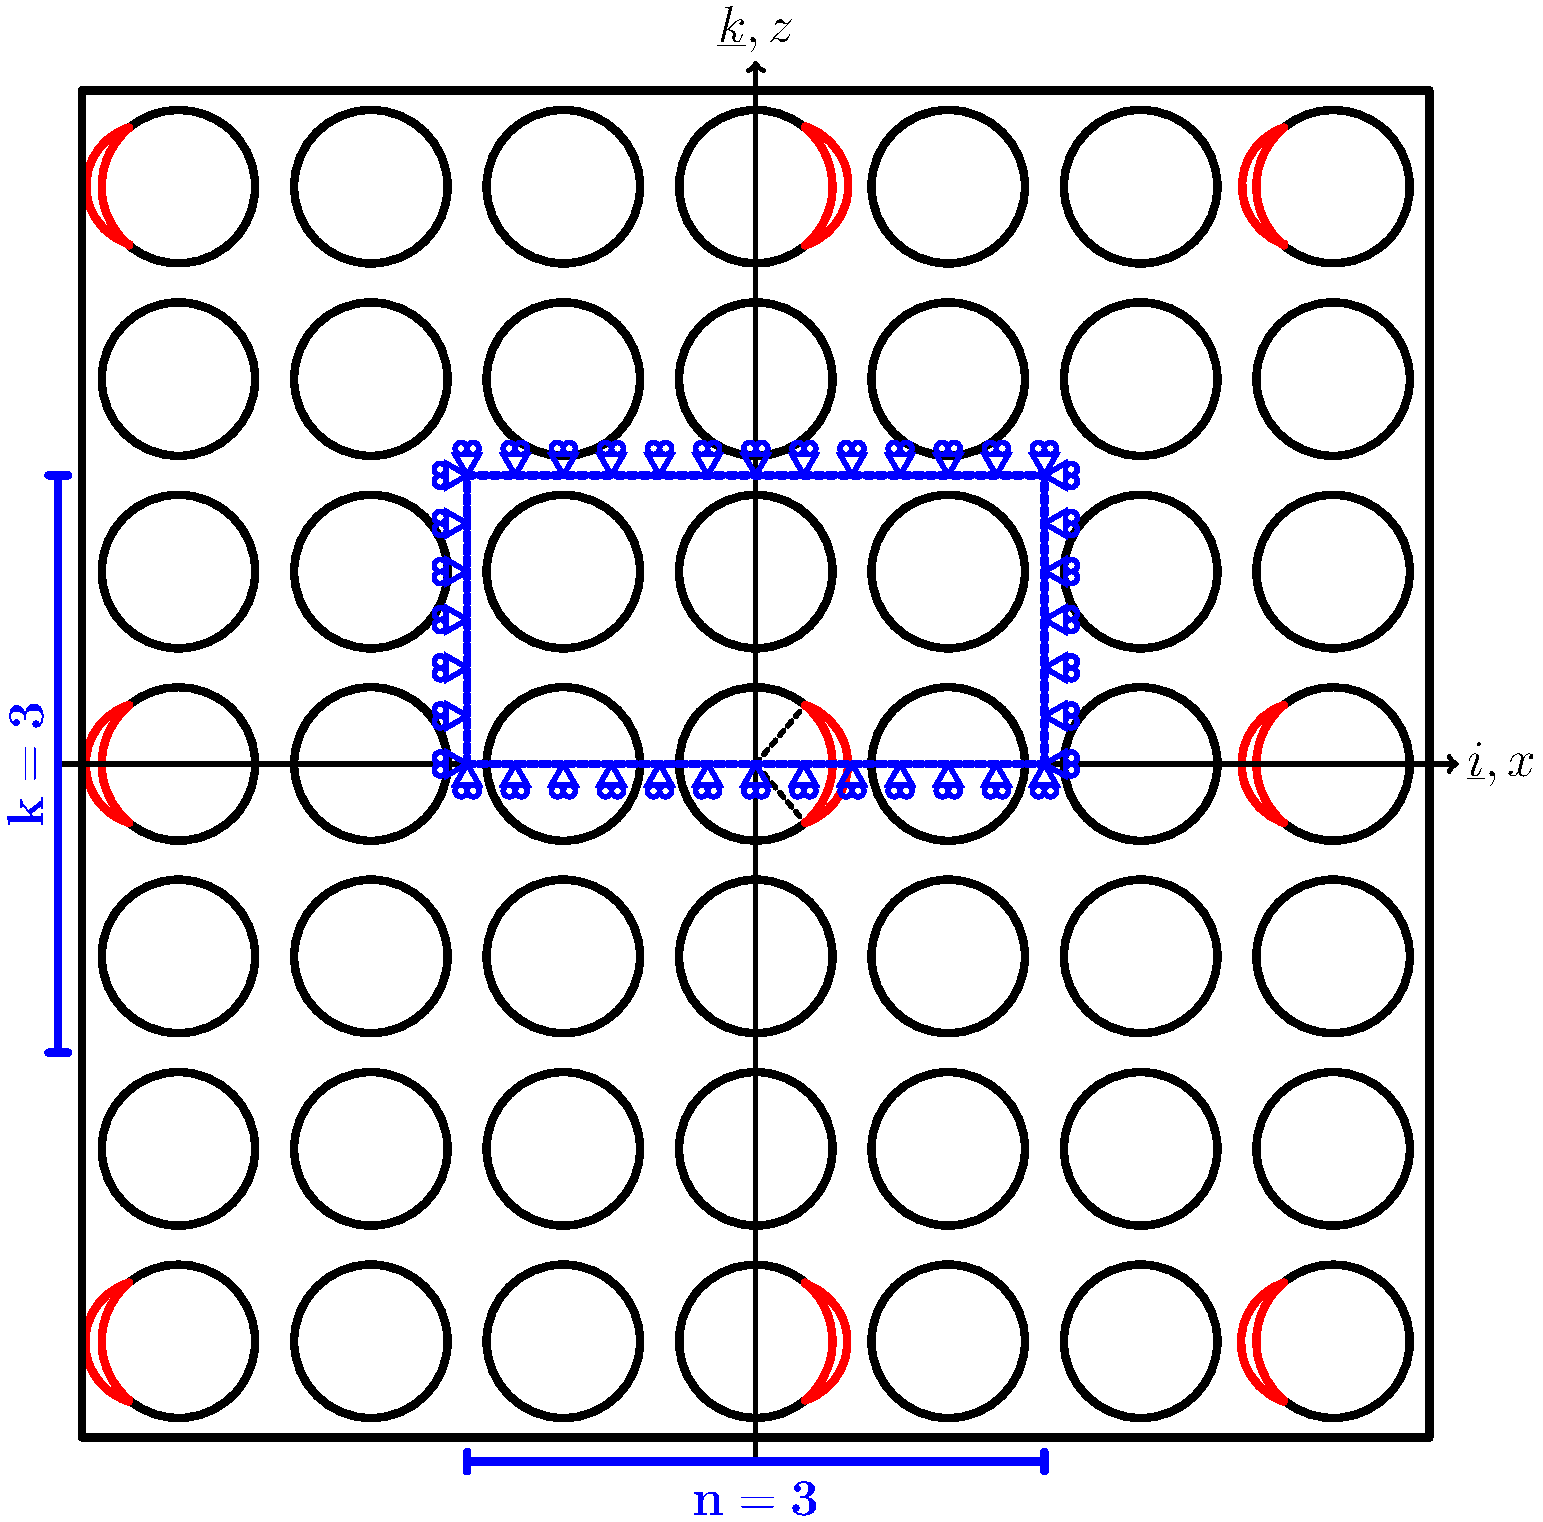
\includegraphics[width=\textwidth]{chesstableArrangement.pdf}
\caption{Rows of fibers with debonds repeating at different distances along the horizontal direction and rows with debonded fibers repeating at different distances along the vertical direction: models $n\times k-coupling$.}\label{fig:laminateModelsA}
\end{figure}

Models in Figures~\ref{fig:laminateModelsB} and~\ref{fig:laminateModelsC} represent instead a UD composite with respectively vertical lines and horizontal rows of partially debonded fibers repeating at the regular intervals respectively in the horizontal and vertical direction, measured respectively in terms of vertical lines and horizontal rows of fully bonded (undamaged) fibers. According to the nomenclature introduced in~\ref{subsec:names}, these two models are identified respectively by $n\times 1-coupling$ and $1\times k-coupling$.

\begin{figure}[!h]
\centering
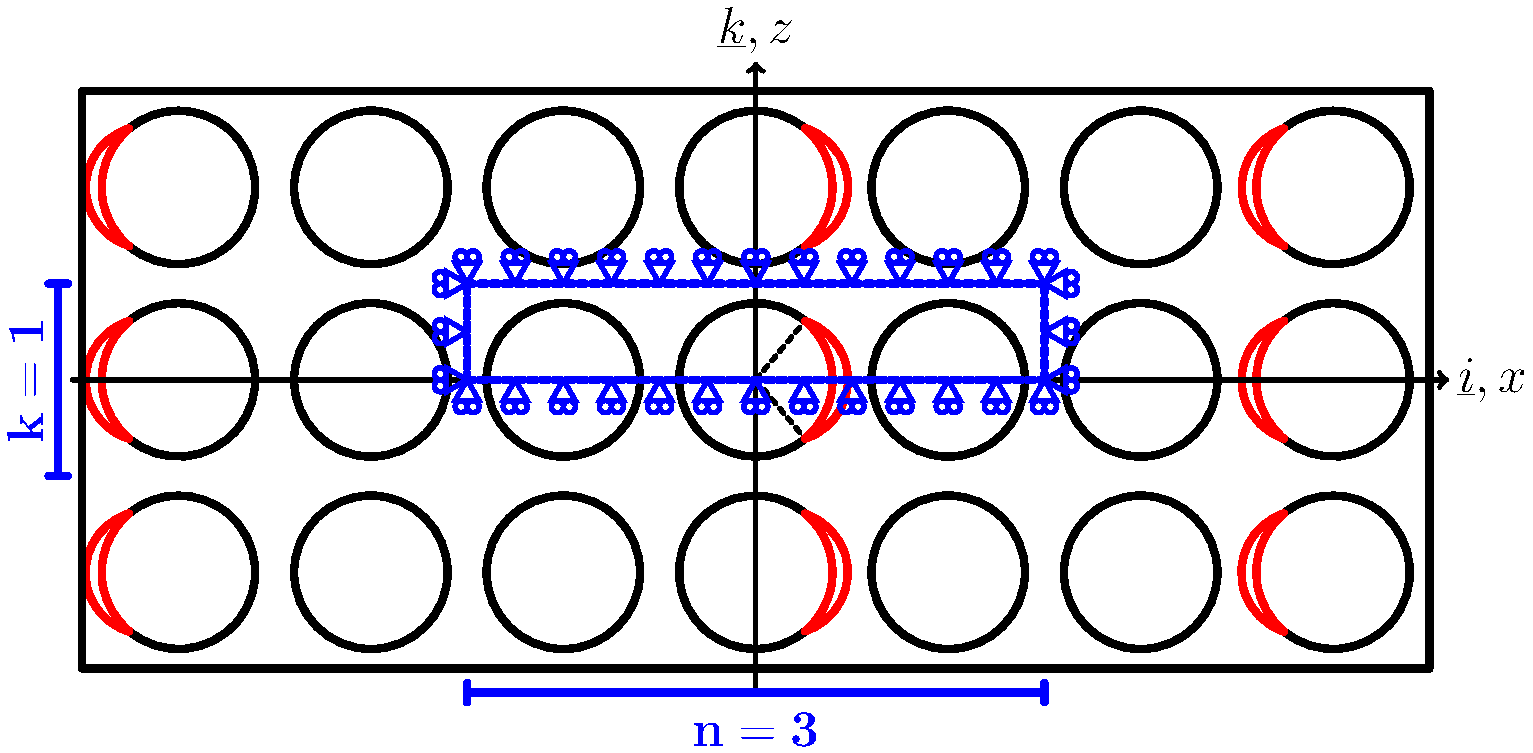
\includegraphics[width=\textwidth]{verticalLinesOfDebonds.pdf}
\caption{Vertical lines of fibers with debonds repeating at different distances along the horizontal direction: models $n\times 1-coupling$.}\label{fig:laminateModelsB}
\end{figure}

Model $n\times 1-coupling$ in Figure~\ref{fig:laminateModelsB} is studied to investigate the interaction of debonds in a configuration that represents, although in an idealized form, the stage preceding coalescence of debonds and formation of macroscopic transverse cracks. 

\begin{figure}[!h]
\centering
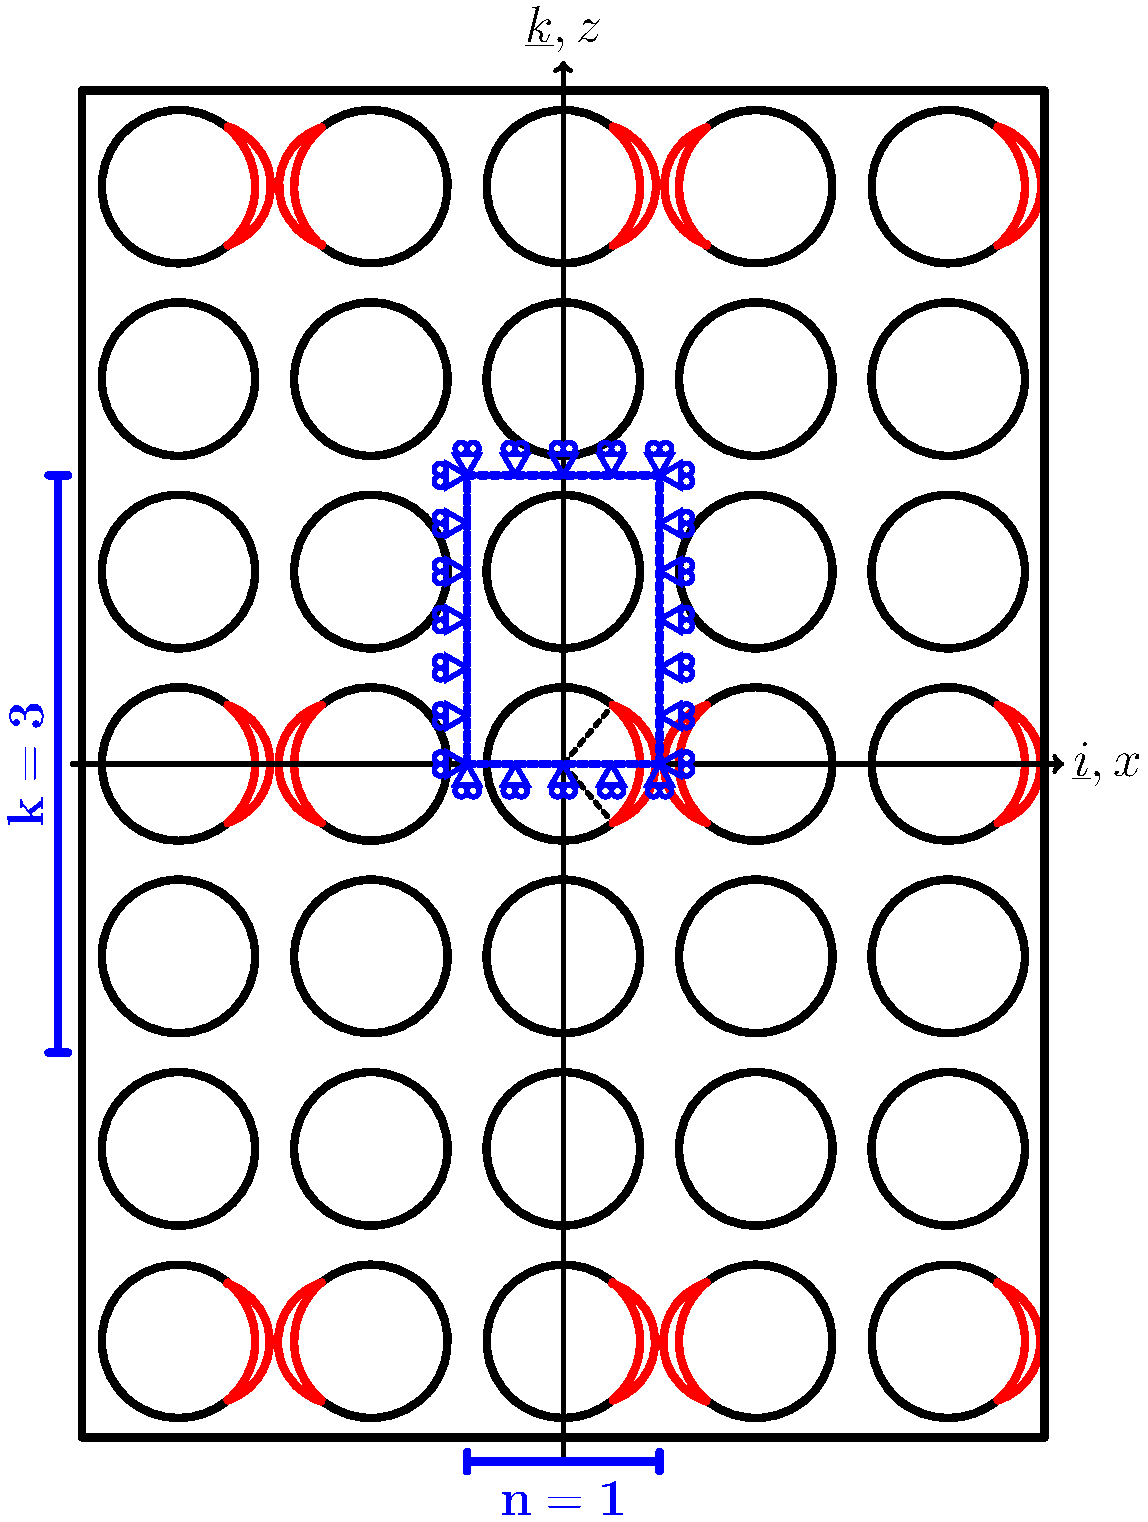
\includegraphics[width=\textwidth]{horizontalDebondLineRepeatingVertically.pdf}
\caption{Horizontal rows of fibers with debonds repeating at different distances along the vertical direction: models $1\times k-coupling$.}\label{fig:laminateModelsC}
\end{figure}

On the other hand, model $n\times 1-coupling$ in Figure~\ref{fig:laminateModelsC} addresses a configuration of debonds that has not been observed in in-situ analyses of UD composites in transverse tension and can thus be deemed unphysical, but has nonetheless the potential to shed light on debonds' interaction mechanisms that makes this configuration unobservable.

\subsection{Finite Element (FE) discretization}

Discretization and analysis of RUCs is performed with the Finite Element Method (FEM) within the Abaqus environment, a commercial FEM software~\cite{abq12}. Length $l$ and height $h$ of the model are respectively determined by the number of fibers $n$ in the horizontal direction and $k$ across the thickness (see~\ref{subsec:rve}) according to Eq.~\ref{eq:lengthheight}:

\begin{equation}\label{eq:lengthheight}
l=2nL\qquad h=kL;
\end{equation}

where $2L$ is the length of a one-fiber unit, see Fig.~\ref{subfig:modelschem}, and $L$ is defined as a function of the fiber volume fraction $V_{f}$ and the fiber radius $R_{f}$ according to

\begin{equation}\label{eq:LVf}
L=\frac{R_{f}}{2}\sqrt{\frac{\pi}{V_{f}}}.
\end{equation}

$R_{f}$ is assumed to be the same for every fiber and equal to $1\ \mu m$. The choice of the previous value is not dictated by physical considerations but for simplicity. It is thus useful to remark here that, in a linear elastic solution as the one considered in the present work, the ERR is proportional to the geometrical dimensions of the model and, consequently, recalculation of the ERR for fibers of any size requires a simple multiplication. Notice also that relationships in Eqs.~\ref{eq:lengthheight} and~\ref{eq:LVf} imply that the local and global $V_{f}$ are everywhere equal.

\begin{figure}[!h]
\centering
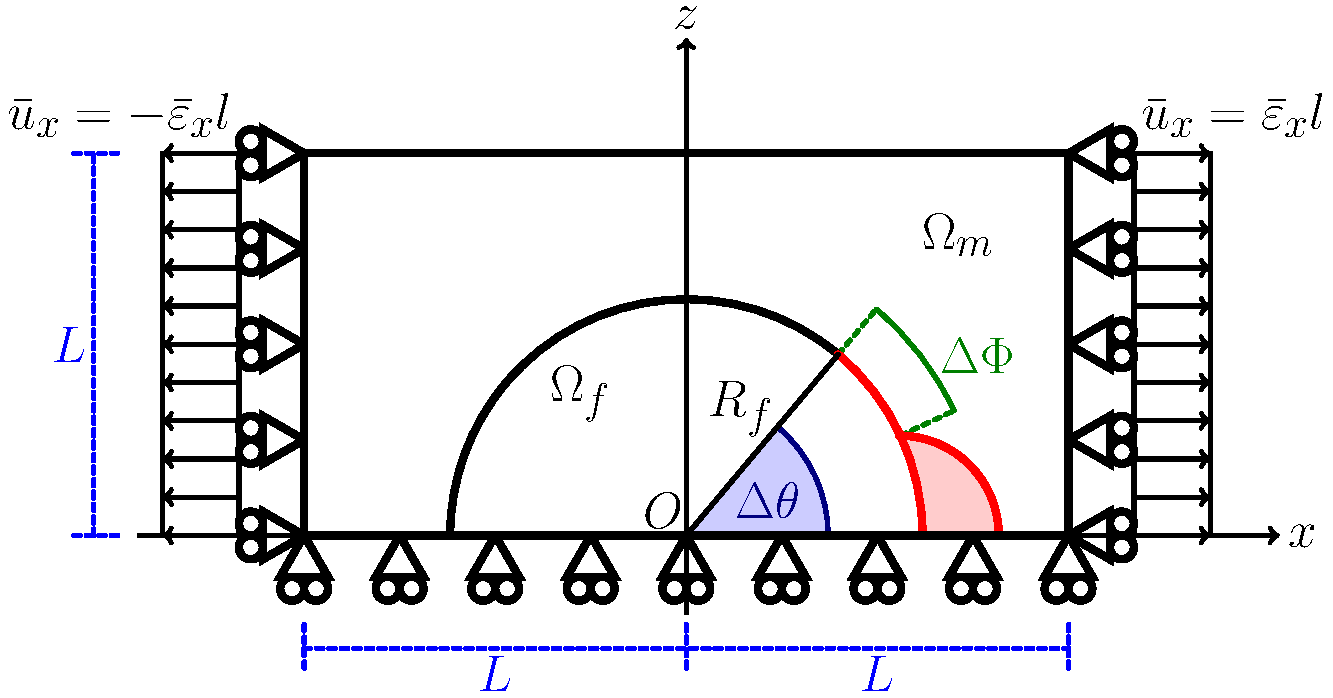
\includegraphics[width=\textwidth]{RUC.pdf}
\caption{Schematic of the model with its main parameters.}\label{fig:modelschem}
\end{figure}

The debond is placed symmetrically with respect to the $x$ axis (see Fig.~\ref{fig:modelschem}) and it is characterized by an angular size of $\Delta\theta$ (making the full debond size equal to $2\Delta\theta$). For large debond sizes (at least $\geq 60^{\circ}-80^{\circ}$), a region $\Delta\Phi$ of variable size appears at the crack tip where the crack faces are in contact with each other but free to slide relatively to each other. In order to model crack faces motion in the contact zone, frictionless contact is considered between the two crack faces to allow free sliding and avoid interpenetration. Symmetry with respect to the $x$ axis is applied on the lower boundary and coupling of vertical displacement on the upper boundary. Kinematic coupling on the $x$-displacement is applied along the left and right sides of the RUC in the form of a constant $x$-displacement $\pm\bar{\varepsilon}_{x} l$, corresponding to transverse strain $\bar{\varepsilon}_{x}$ equal to $1\%$.

\begin{table}[!htbp]
 \centering
 \caption{Summary of the mechanical properties of fiber and matrix. $E$ stands for Young's modulus, $\mu$ for shear modulus and $\nu$ for Poisson's ratio.}
 \begin{tabular}{cccc}
\textbf{Material} & \textbf{$E\left[GPa\right]$}\ & \textbf{$\mu\left[GPa\right]$} & \textbf{$\nu\left[-\right]$} \\
\midrule
Glass fiber    & 70.0  & 29.2   & 0.2  \\
Epoxy    & 3.5    & 1.25   & 0.4
\end{tabular}
\label{tab:phaseprop}
\end{table}

Meshing of the model is accomplished with second order, 2D, plane strain triangular (CPE6) and quadrilateral (CPE8) elements. A regular mesh of 8-node ($2^{nd}$ order rectangular) elements with almost unitary aspect ratio is enforced at the crack tip in order to ensure the convergence of the ERR. The angular size $\delta$ of an element in the crack tip neighborhood is always equal to $0.05^{\circ}$. The crack faces are modeled as element-based surfaces and a small-sliding contact pair interaction with no friction is imposed between them. The Mode I, Mode II and total Energy Release Rates (ERRs) (respectively referred to as $G_{I}$, $G_{II}$ and $G_{TOT}$) are the main result of FEM simulations; they are evaluated using the VCCT~\cite{Krueger2004} implemented in a in-house Python routine and, for $G_{TOT}$ only, the J-integral~\cite{Rice1968} is calculated by use of the Abaqus built-in command. A glass fiber-epoxy UD composite is treated in the present work, and it is assumed that their response lies always in the linear elastic domain. The material properties of glass fiber and epoxy are reported in Table~\ref{tab:phaseprop}. Validation is performed with respect to the results reported in~\cite{Paris2007,Sandino2016}, which were obtained with the Boundary Element Method (BEM) for a model of a single fiber with a symmetric debond placed in an infinite matrix. As discussed in more detail in~\cite{DiStasio2019}, the agreement between FEM (present work) and BEM~\cite{Paris2007,Sandino2016} solutions is good and the difference between the two does not exceed $5\%$. This provides us with a level of uncertainty with which we can analyze the significance of observed trends: any relative difference in ERR between different RUCs smaller than $5\%$ cannot be reliably distinguished from numerical uncertainty and its discussion should thus be avoided.

\section{Results \& Discussion}

\subsection{Interaction between isolated debonds in infinite UD composites}\label{subsec:chesstable}

The effect on Mode I and Mode II ERR of the interaction between debonds appearing at regular distances (in terms of fully bonded fibers) in the horizontal and vertical directions (models $n\times k-coupling$) is shown respectively in Figure~\ref{fig:debonddebondGI} and Figure~\ref{fig:debonddebondGII}. It can be observed that it is the distance between debonds in the horizontal direction that presents a relevant effect on ERR: the number of fully bonded fibers between consecutive debonds in the vertical direction has a negligible influence on Mode I and a very modest effect, below or at the limit of the $5\%$ accuracy of the model, on Mode II.

\begin{figure}[!h]
\centering
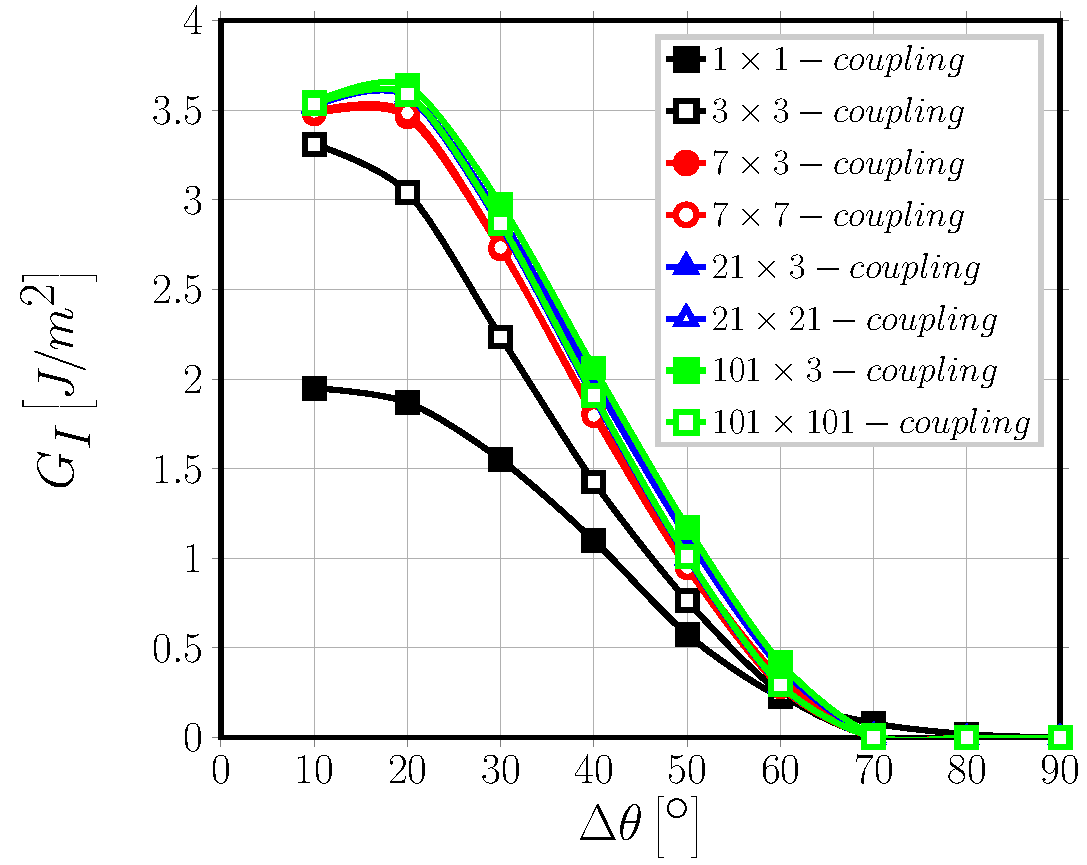
\includegraphics[width=\textwidth]{nxk-coupling-vf60-GI.pdf}
\caption{Effect of debond-debond interaction in infinite UD composites on Mode I ERR: models $n\times k-coupling$. $V_{f}=60\%$, $\varepsilon_{x}=1\%$.}\label{fig:debonddebondGI}
\end{figure}

On the other hand, increasing the number of fully bonded fibers between debonds in the horizontal direction leads to a significant increase in both Mode I and Mode II ERR, due to the magnification of the $x$-strain in the crack tip neighborhood~\cite{DiStasio2019}. A critical distance (in terms of undamaged fibers) at which a non-interacting solution can be observed is apparent for Mode I (Figure~\ref{fig:debonddebondGI}). Given that Mode II ERR for models $21\times 3-coupling$, $21\times 21-coupling$, $101\times 3-coupling$ and $101\times 101-coupling$ is in a $\leq5\%$ range with respect to each other and thus their difference is not significant taking into account model accuracy, it can be argued that also in Mode II a critical distance exists at which a non-interacting solution appears.

\begin{figure}[!h]
\centering
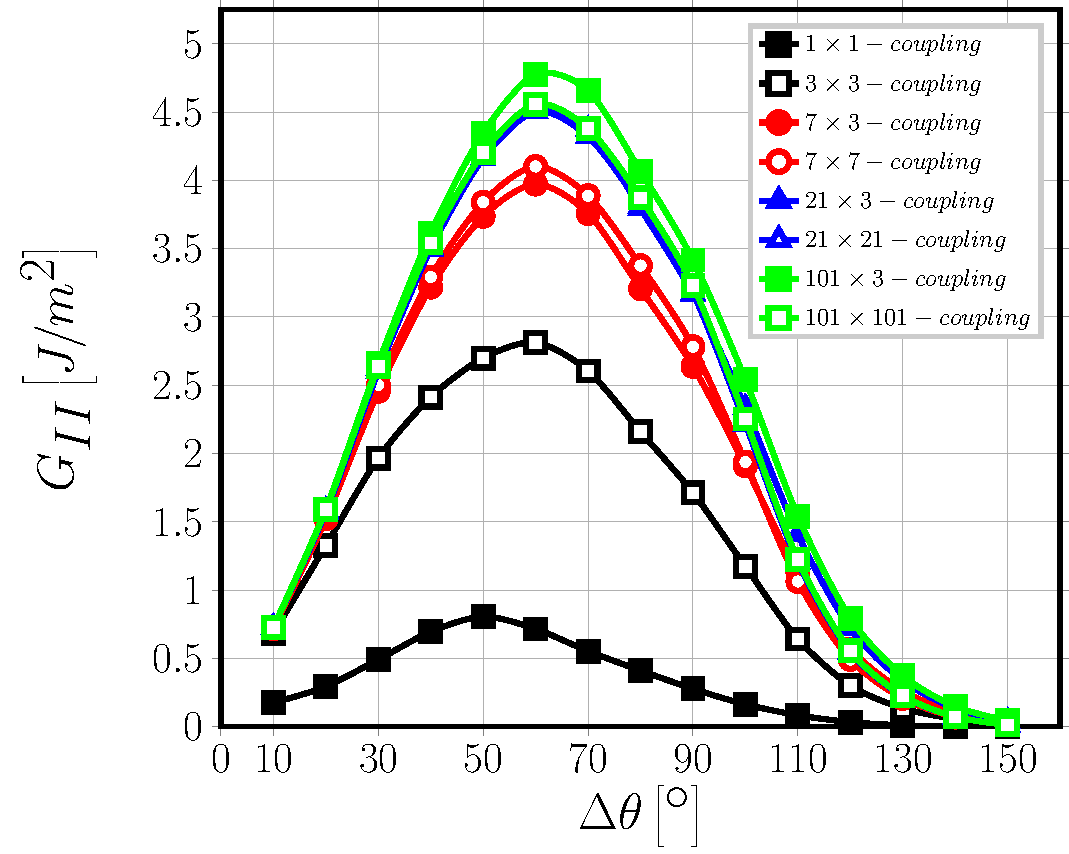
\includegraphics[width=\textwidth]{nxk-coupling-vf60-GII.pdf}
\caption{Effect of debond-debond interaction in infinite UD composites on Mode II ERR: models $n\times k-coupling$. $V_{f}=60\%$, $\varepsilon_{x}=1\%$.}\label{fig:debonddebondGII}
\end{figure}

\subsection{Debond-debond interaction between vertical lines of partially debonded fibers in infinite UD composites}

The results presented in Figures~\ref{fig:horizontalGI} and~\ref{fig:horizontalGII} for respectively Mode I and Mode II ERR of models $1\times k-coupling$ confirm the observations presented in Section~\ref{subsec:chesstable}. Models $1\times k-coupling$ represents the RVE of an infinite UD composite with horizontal fiber rows that appear at regular intervals (measured in terms of fully bonded fibers) and in which fibers are all partially debonded (see Fig.~\ref{fig:laminateModelsC} for reference).

\begin{figure}[!h]
\centering
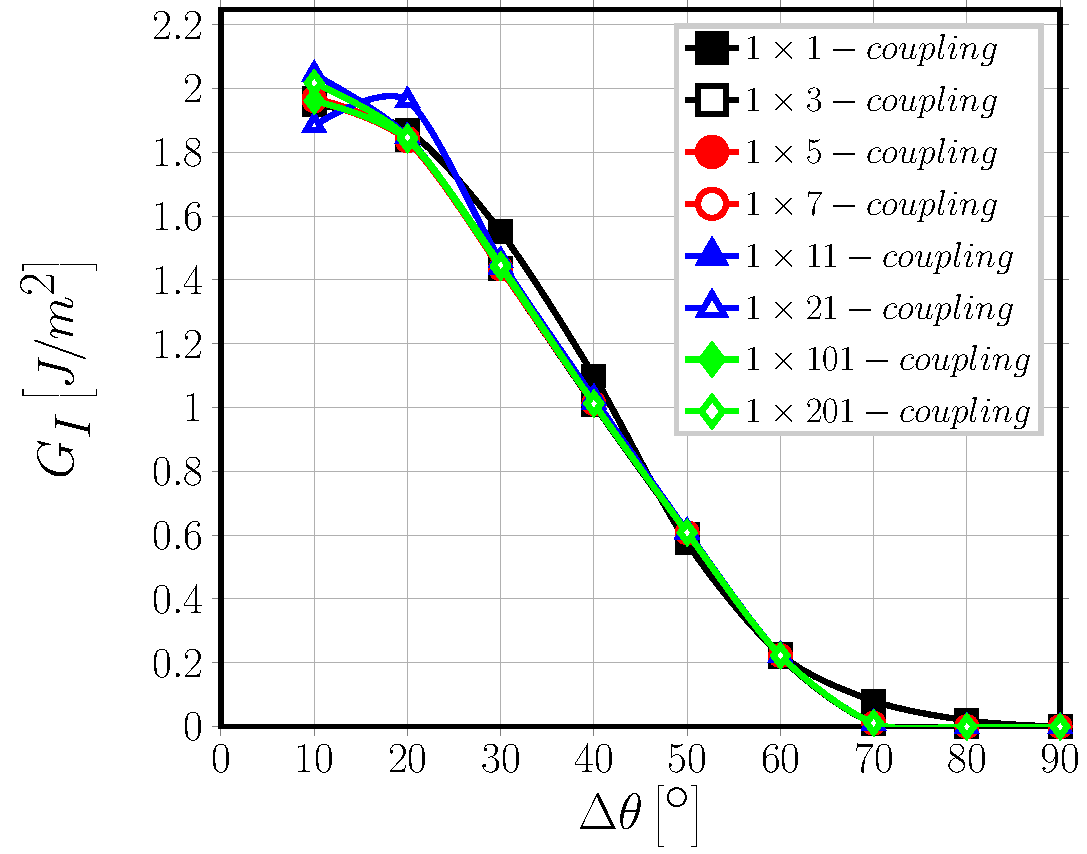
\includegraphics[width=\textwidth]{1xk-coupling-vf60-GI.pdf}
\caption{Effect of debond-debond interaction in infinite UD composites on Mode I ERR: models $1\times k-coupling$. $V_{f}=60\%$, $\varepsilon_{x}=1\%$.}\label{fig:horizontalGI}
\end{figure}

Varying the number $k$ of undamaged fibers between fiber rows of only partially debonded fibers does not have any effect on ERR, neither in Mode I (Figure~\ref{fig:horizontalGI}) nor in Mode II (Figure~\ref{fig:horizontalGII}). The observations of Sec.~\ref{subsec:chesstable} are thus confirmed: it is the presence of fully bonded fibers only in the horizontal direction, i.e. the loading direction, that affects the debond ERR through $x$-strain magnification.

\begin{figure}[!h]
\centering
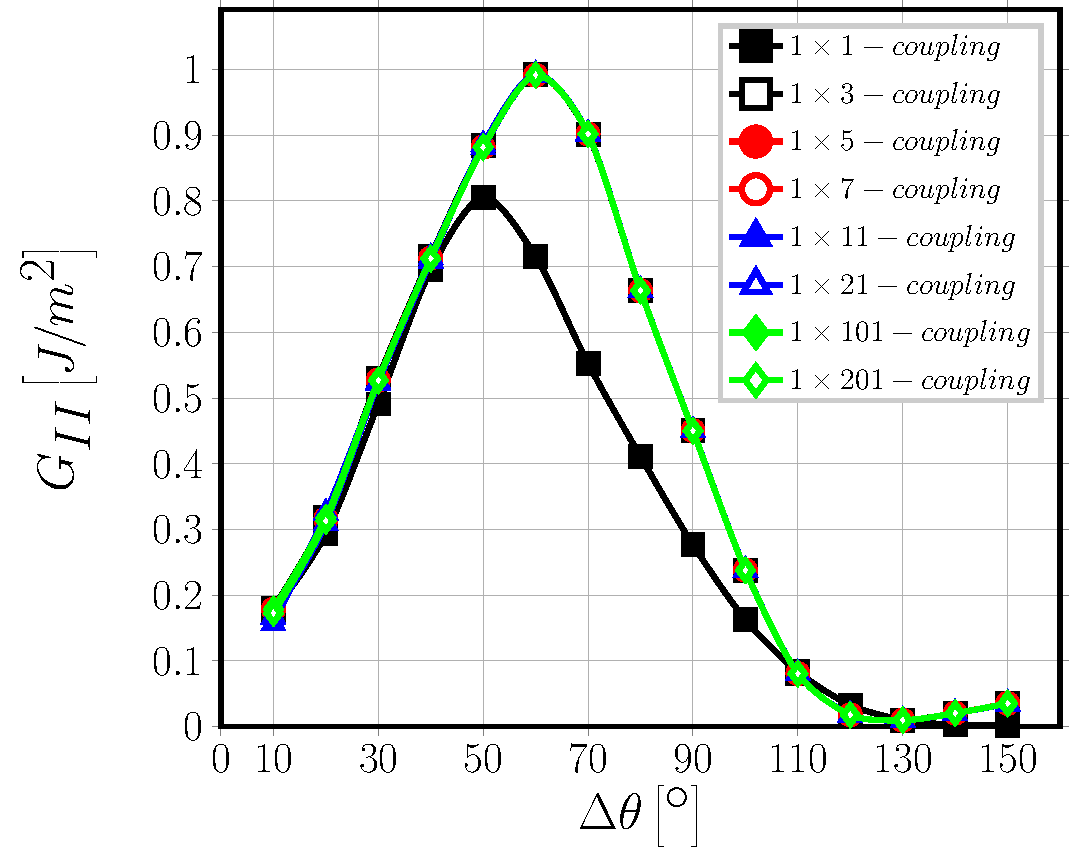
\includegraphics[width=\textwidth]{1xk-coupling-vf60-GII.pdf}
\caption{Effect of debond-debond interaction in infinite UD composites on Mode II ERR: models $1\times k-coupling$. $V_{f}=60\%$, $\varepsilon_{x}=1\%$.}\label{fig:horizontalGII}
\end{figure}

\subsection{Debond-debond interaction between horizontal rows of partially debonded fibers in infinite UD composites}

Figures~\ref{fig:verticalGI} and~\ref{fig:verticalGII} report respectively Mode I and Mode II ERR for models $1\times k-coupling$, which correspond to the RVEs of UD composites with vertical lines of partially debonded fibers appearing at regular intervals (in terms of undamaged fibers) in the horizontal direction (see Fig.~\ref{fig:laminateModelsB} for reference). 

\begin{figure}[!h]
\centering
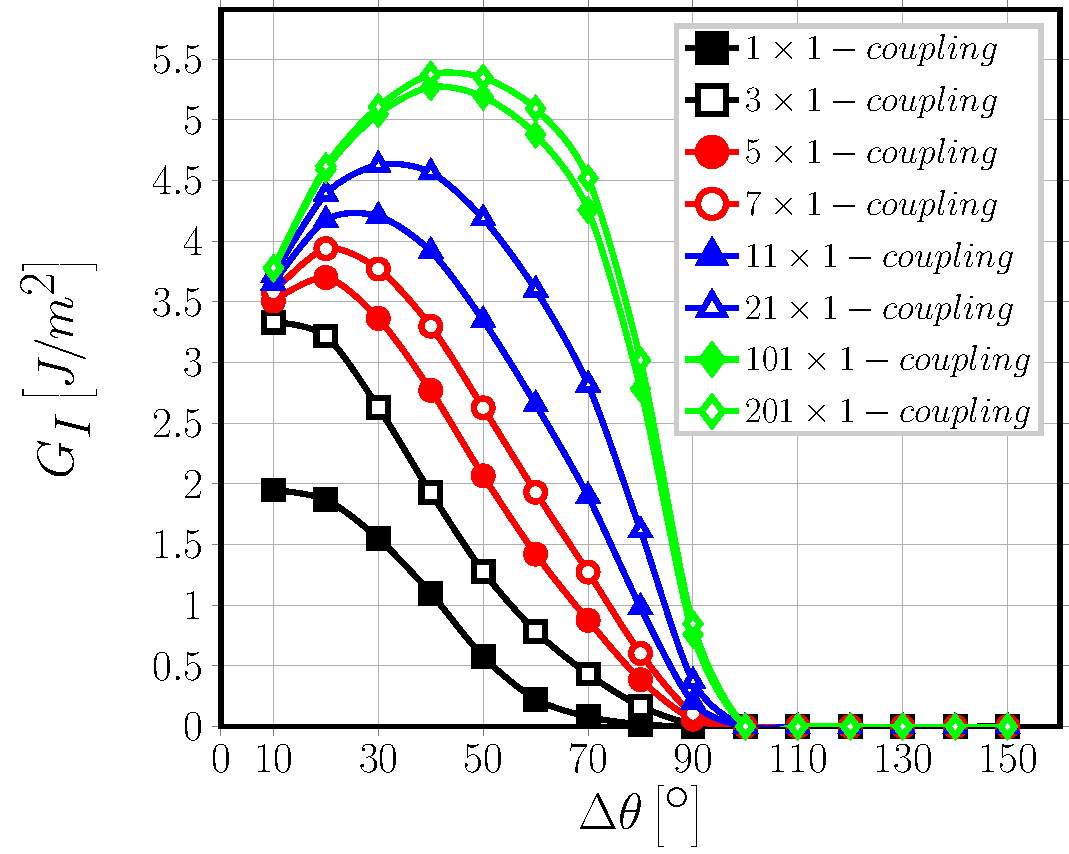
\includegraphics[width=\textwidth]{nx1-coupling-vf60-GI.pdf}
\caption{Effect of debond-debond interaction in infinite UD composites on Mode I ERR: models $n\times 1-coupling$. $V_{f}=60\%$, $\varepsilon_{x}=1\%$.}\label{fig:verticalGI}
\end{figure}

\begin{figure}[!h]
\centering
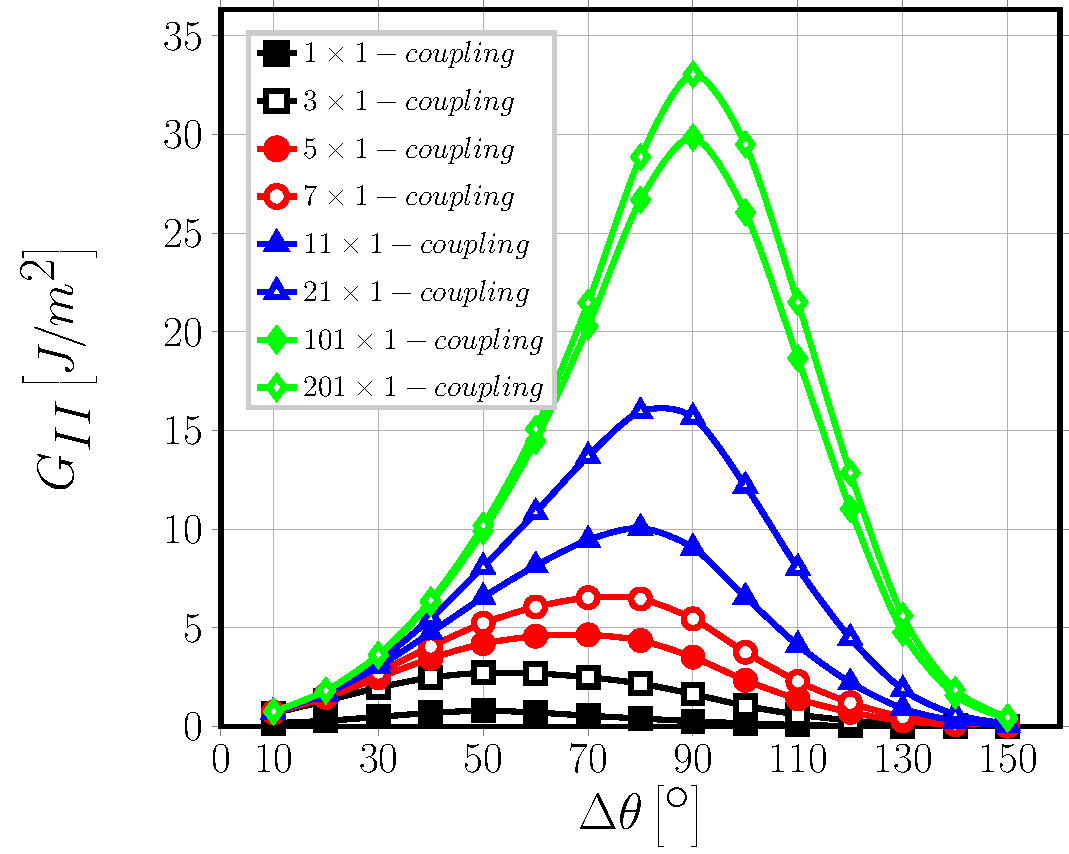
\includegraphics[width=\textwidth]{nx1-coupling-vf60-GII.pdf}
\caption{Effect of debond-debond interaction in infinite UD composites on Mode II ERR: models $n\times 1-coupling$. $V_{f}=60\%$, $\varepsilon_{x}=1\%$.}\label{fig:verticalGII}
\end{figure}

\section{Conclusions \& Outlook}

From the observations made in the previous section, it seems reasonable to derive the following conclusions about the growth of debonds in UD composites:

\begin{itemize}
\item at given strain level, multiple debonds can appear on not consecutive vertically-aligned fibers;
\item at a given strain level, the vertical lines of fibers on which debonds grow are determined by the horizontal distance from pre-existing debonds;
\item a minimum non-interactive distance exists for the Energy Release Rate;
\item when spacing between vertical lines of debonds is lower than the minimum non-interactive distance, the ERR decreases;
\item thus, conversely, when spacing between vertical lines of debonds is lower than the minimum non-interactive distance, higher levels of strain are needed to grow debonds;
\end{itemize}


\section*{Acknowledgements}

Luca Di Stasio gratefully acknowledges the support of the European School of Materials (EUSMAT) through the DocMASE Doctoral Programme and the European Commission through the Erasmus Mundus Programme.

\bibliography{refs}

\end{document}
